\newpage
\section{Theorie und Vorwissen}
\subsection{Zephyr}
    Zephyr ist ein Open-Source-Echtzeitbetriebssystem welches von der Linux Foundation.\footnote{Quelle: \url{https://de.wikipedia.org/wiki/Zephyr_(Betriebssystem)}}
    Ein Echtzeitbetriebssystem, real-time operating system \textbf{RTOS} ist ein Betriebssystem, das Echtzeit-Anforderungen erfüllen kann. 
    Das bedeutet, dass Anfragen eines Anwendungsprogramms innerhalb einer Voraus bestimmbaren Zeit gesichert verarbeitet werden.\footnote{Quelle: \url{https://de.wikipedia.org/wiki/Echtzeitbetriebssystem}}
    \\
    Zephyr wurde mit dem \href{https://docs.zephyrproject.org/latest/getting_started/index.html}{Getting-Started-GUID} Linux Subsystem von Windows installiert. 
    Um ein Zephyr Projekt zu kompilieren wird Zephyr eigenes \textbf{West}\footnote{\url{https://docs.zephyrproject.org/2.4.0/guides/west/index.html}} verwendet.\\
    \textbf{West} ist ein Kompilierungs-Tool von Zephyr. Es verwendet Ninja und CMake um das Projekt zu kompilieren. 
    West wird folgendermaßen verwendet, um ein Projekt zu kompilieren: 
    \begin{lstlisting}[style=StyleC, captionpos=b, caption=West Beispiel, label=West Beispiel]
west build -p auto -b nativ_posix_64 
    \end{lstlisting}

    \subsubsection{west}
        \subsubsubsection{West als Repo Verwalter}
            West ist ein Command-line tool von Zephyr. Es wird unabhängig von Zephyr installiert und wird zur Kompilierung und Flashen verwendet. 
            Das Problem das bei solchen Projekten entsteht ist, dass es sich aus mehreren GIT Repositories mit unterschiedlichen Versionen zusammen setzen kann, somit
            muss dafür gesorgt werden, dass alle GIT Repositories, mit der korrekter Version im korrekten pfad sich befinden. 
            Diese werden im sogenannten \textit{west manifest} \textbf{west.yaml} festgelegt.\footnote{\url{https://docs.zephyrproject.org/latest/guides/west/index.html}}
            \begin{lstlisting}[style=StylePython, captionpos=b, caption=west.yaml]
manifest:
defaults:
    remote: upstream

remotes:
    - name: upstream
    url-base: https://github.com/zephyrproject-rtos

#
# Please add items below based on alphabetical order
projects:
    - name: cmsis
    revision: c3bd2094f92d574377f7af2aec147ae181aa5f8e
    repo-path: mcuboot
    path: modules/tee/tfm-mcuboot
    revision: 1.7.0-rc1
    ...
self:
    path: zephyr
    west-commands: scripts/west-commands.yml    
            \end{lstlisting} 
            Um einen Ordner zu initialisieren wird \textbf{west init} und zum downloaden der Daten \textbf{west update} verwendet.\footnote{\url{https://github.com/zephyrproject-rtos/west}}
        \subsubsubsection{West als Compiler}
            West ist der Haupt-Compiler von Zephyr, west ruft cmake, ninja oder make im Hintergrund auf um erfolgreich zu Kompilieren. 
            Im Hintergrund wird hauptsächlich ninja verwendet.\footnote{\url{https://docs.zephyrproject.org/latest/application/index.html?highlight=ninja}}


\newpage
    \subsubsection{ninja}
        Ninja ist ein kleines build System mit Fokus auf Geschwindigkeit. 
        Es wird in assembler geschrieben und ist so designend, dass die Input files von einem höheren Build-System erstellt werden (west) und das es so schnell wie möglich builded. 
        

        % Why yet another build system?
        % Where other build systems are high-level languages Ninja aims to be an assembler.
        
        % Ninja build files are human-readable but not especially convenient to write by hand. (See the generated build file used to build Ninja itself.) These constrained build files allow Ninja to evaluate incremental builds quickly.
        
        % Should you use Ninja?
        % Ninja's low-level approach makes it perfect for embedding into more featureful build systems; see a list of existing tools. Ninja is used to build Google Chrome, parts of Android, LLVM, and can be used in many other projects due to CMake's Ninja backend.
        
        % See the manual for more: philosophical background, whether and how you can use Ninja for your project, platform support, and details about the language semantics.

    \subsubsection{KConfig}
    \textbf{Kernel Configuration File}\footnote{\url{https://docs.zephyrproject.org/latest/application/index.html?\#application-kconfig}}ist die \textcolor{red}{prj.conf} Datei in einem 
    Zephyr Projekt. In diesem werden besstimmte Konfigurationen, Funktionen und \anfuehrung{Geräte}, wie z.b. \textit{CONFIG\_SERIAL=y} aktiviert. 
% The Zephyr kernel and subsystems can be configured at build time to adapt them for specific application and platform needs. Configuration is handled through Kconfig, which is the same configuration system used by the Linux kernel. The goal is to support configuration without having to change any source code.
% Configuration options (often called symbols) are defined in Kconfig files, which also specify dependencies between symbols that determine what configurations are valid. Symbols can be grouped into menus and sub-menus to keep the interactive configuration interfaces organized.
% The output from Kconfig is a header file autoconf.h with macros that can be tested at build time. Code for unused features can be compiled out to save space.
% The following sections explain how to set Kconfig configuration options, go into detail on how Kconfig is used within the Zephyr project, and have some tips and best practices for writing Kconfig files.

\newpage
    \subsubsection{Device Tree}
    Der Device Tree\footnote{\url{https://docs.zephyrproject.org/latest/guides/dts/intro.html}\\\url{https://docs.zephyrproject.org/latest/reference/devicetree/index.html\#devicetree}} ist 
    in einem Zephyr Projekt eine Datei mit der Endung \textbf{.dts} dort stehen alle für das ausgewählte Board verfügbare Geräte drinnen.
    Im Fall des nativ\_posix\_64 sieht dieses folgendermaßen aus. 
    \begin{lstlisting}[style=StyleC, captionpos=b, caption=West Beispiel, label=West Beispiel]
/dts-v1/;

/ {
    #address-cells = < 0x1 >;
    #size-cells = < 0x1 >;
    model = "Native POSIX Board";
    compatible = "zephyr,posix";
    chosen {
        zephyr,console = &uart0;
        zephyr,shell-uart = &uart0;
        zephyr,uart-mcumgr = &uart0;
        zephyr,flash = &flash0;
        zephyr,entropy = &rng;
        zephyr,flash-controller = &flashcontroller0;
        zephyr,ec-host-interface = &hcp;
    };
    aliases {
        eeprom-0 = &eeprom0;
        i2c-0 = &i2c0;
        spi-0 = &spi0;
        led0 = &led0;
    };
    leds {
        compatible = "gpio-leds";
        led0: led_0 {
            gpios = < &gpio0 0x0 0x0 >;
            label = "Green LED";
        };
    };

    ...

    };
    uart0: uart {
        status = "okay";
        compatible = "zephyr,native-posix-uart";
        label = "UART_0";
        current-speed = < 0x0 >;
    };
    
    ...

};    
    \end{lstlisting}


\newpage
    \subsubsection{Tinycrypt}
    Die TinyCrypt-Bibliothek bietet eine Implementierung für eingeschränkte Geräte von minimalen Standard-Kryptographie-Grundelementen.
    Di Bibliothek ist von Intel\footnote{\url{https://github.com/intel/tinycrypt}} und wurde in zephyr mit der implementiert.\footnote{\url{https://docs.zephyrproject.org/2.3.0/guides/crypto/tinycrypt.html?highlight=tinycrypt}} 
    Innerhalb von Zephyr können die eignenen Crypto API Befehle oder die direkten TinyCrypt Befehle verwendet werden. 

     
\subsection{Linux Pseudoterminal}
Ein Pseudoterminal ist ein Dienst der eine bidirektionale Pipe, aufbaut. Sie werden verwendet um ein physisches Terminal zu emulieren. 
Im Fall von Zephyr mit dem nativ\_posx Board wird ein Pseudoterminal verwendet um mit dem Baord zu kommunizieren. Der Pfad dieses Terminals ist /dev/pts/.
\subsection{Threads}
Innerhalb eines Betriebssystems werden Applikationen und Abläufe als Prozesse realisiert. Prozesse werden vom Schedular verwaltet. Um nun die Abarbeitung dieser Prozesse zu 
beschleunigen, besteht ein ein Prozess aus mehreren parallel laufenden Threads. Diese Threads beinhalten einen Teil des Prozesses, dadurch können große Probleme bestehen. 
Es muss sichergestellt werden, dass Threads nie auf die gleichen Variablen/Ressourcen zugreifen, da ansonsten Race-Conditions entstehen. 
\begin{figure}[!htb]
    \centering
    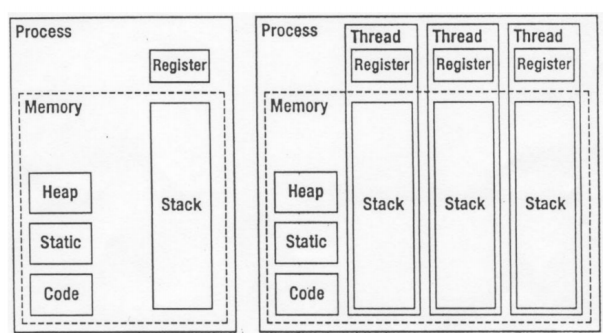
\includegraphics[width=0.65\linewidth]{Process-Threads.png}
    \caption{Process-Threads}
    \label{caption:Process-Threads}
\end{figure}

\newpage
\subsection{Message-Queue}
Eine Message-Queue ist ein besonderer Buffer, ein FIFO-Buffer (First-In-First-Out-Buffer). Das bedeutet, es werden Nachrichten in einer Reihe in den Buffer geschrieben und es kann nur die
erste Nachricht in der Reihe herausgenommen werden, dabei wird diese nachricht im Buffer gelöscht und die nächste Nachricht rückt nach. 
Solche Message-Queues werden verwendet, um zwischen Threads die Daten korrekt auszutauschen. Da eine Nachricht beim auslesen gelöscht wird, können nicht mehrere Threads gleichzeitig auf 
die Nachricht zugreifen. 
\begin{figure}[!ht]
    \centering
    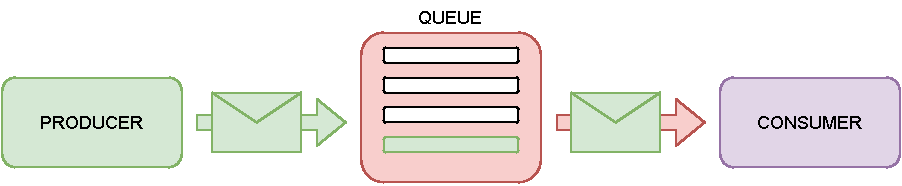
\includegraphics[width=\linewidth]{Message-Queue.pdf}
    \caption{Message-Queue-Darstellung}
    \label{fig:Message-Queue-Darstellung}
\end{figure}